% =============================================================================
% Appendix (MatchIntel2 / MHLC)
% Style inspired by ref.txt: overview index, Parts with \clearpage between them.
% =============================================================================

\section*{Appendix Overview}
\label{app:overview}

This appendix collects the detailed dataset formulation, experiment setup, case studies, limitations, and auxiliary rules referenced in the main paper. We organize the material into the following parts for navigation.

\paragraph{Part A: Detailed Dataset Formulation.}
\begin{itemize}
    \item \textbf{A.} Raw feature definitions (Appendix~\ref{app:raw_features}).
    \item \textbf{B.} The 12 playing-style labels (Appendix~\ref{app:twelve_styles}).
    \item \textbf{C.} Data statistics (Appendix~\ref{app:data_stats}).
    \item \textbf{D.} Construction pipeline (Appendix~\ref{app:construction_pipeline}).
\end{itemize}

\paragraph{Part B: Experiment Setup.}
\begin{itemize}
    \item \textbf{E.} Models: PEFT fine-tuning of LLMs and traditional architecture models trained from scratch (Appendix~\ref{app:models}).
    \item \textbf{F.} Parameters: generation, PEFT, and training-from-scratch settings (Appendix~\ref{app:parameters}).
    \item \textbf{G.} Zero-shot and few-shot prompt templates (Appendix~\ref{app:prompts_zeroshot_fewshot}).
\end{itemize}

\paragraph{Part C: Case Studies.}
\begin{itemize}
    \item \textbf{H.} Qualitative failure cases and representative examples (Appendix~\ref{app:Case Studies}).
\end{itemize}

\paragraph{Part D: Limitations \& Future Work.}
\begin{itemize}
    \item \textbf{I.} Limitations (Appendix~\ref{app:limitations}).
    \item \textbf{J.} Future work (Appendix~\ref{app:future_work}).
\end{itemize}

\paragraph{Part E: U/S/R Error Attribution (auxiliary).}
\begin{itemize}
    \item \textbf{K.} Rule-level definitions for U/S/R discussion and log-based attribution (Appendix~\ref{sec:usrules}).
\end{itemize}

% -----------------------------------------------------------------------------
% \clearpage

\section{Detailed Dataset Formulation}
\label{app:dataset_formulation}

\textbf{The necessity of constructing this dataset:} Existing multimodal datasets are still largely confined to low-level mechanical processing. Fundamentally, they map low-level inputs to other low-level outputs, making it difficult to evaluate whether LLMs can derive high-level conclusions by perceiving the underlying logic behind these data.

\textbf{The reliability of the data source:} This dataset is collected from WhoScored, a leading professional football analysis website. As an authoritative source widely used in sports analytics research \cite{li2022emergent,liu2025can,mahowald2024dissociating}, WhoScored relies on domain experts to maintain high-fidelity match annotations, making it a suitable source for evaluating HWI-related capabilities of LLMs.

\subsection{Raw Feature Definitions}
\label{app:raw_features}

\begin{figure}[!t]
	\centering
	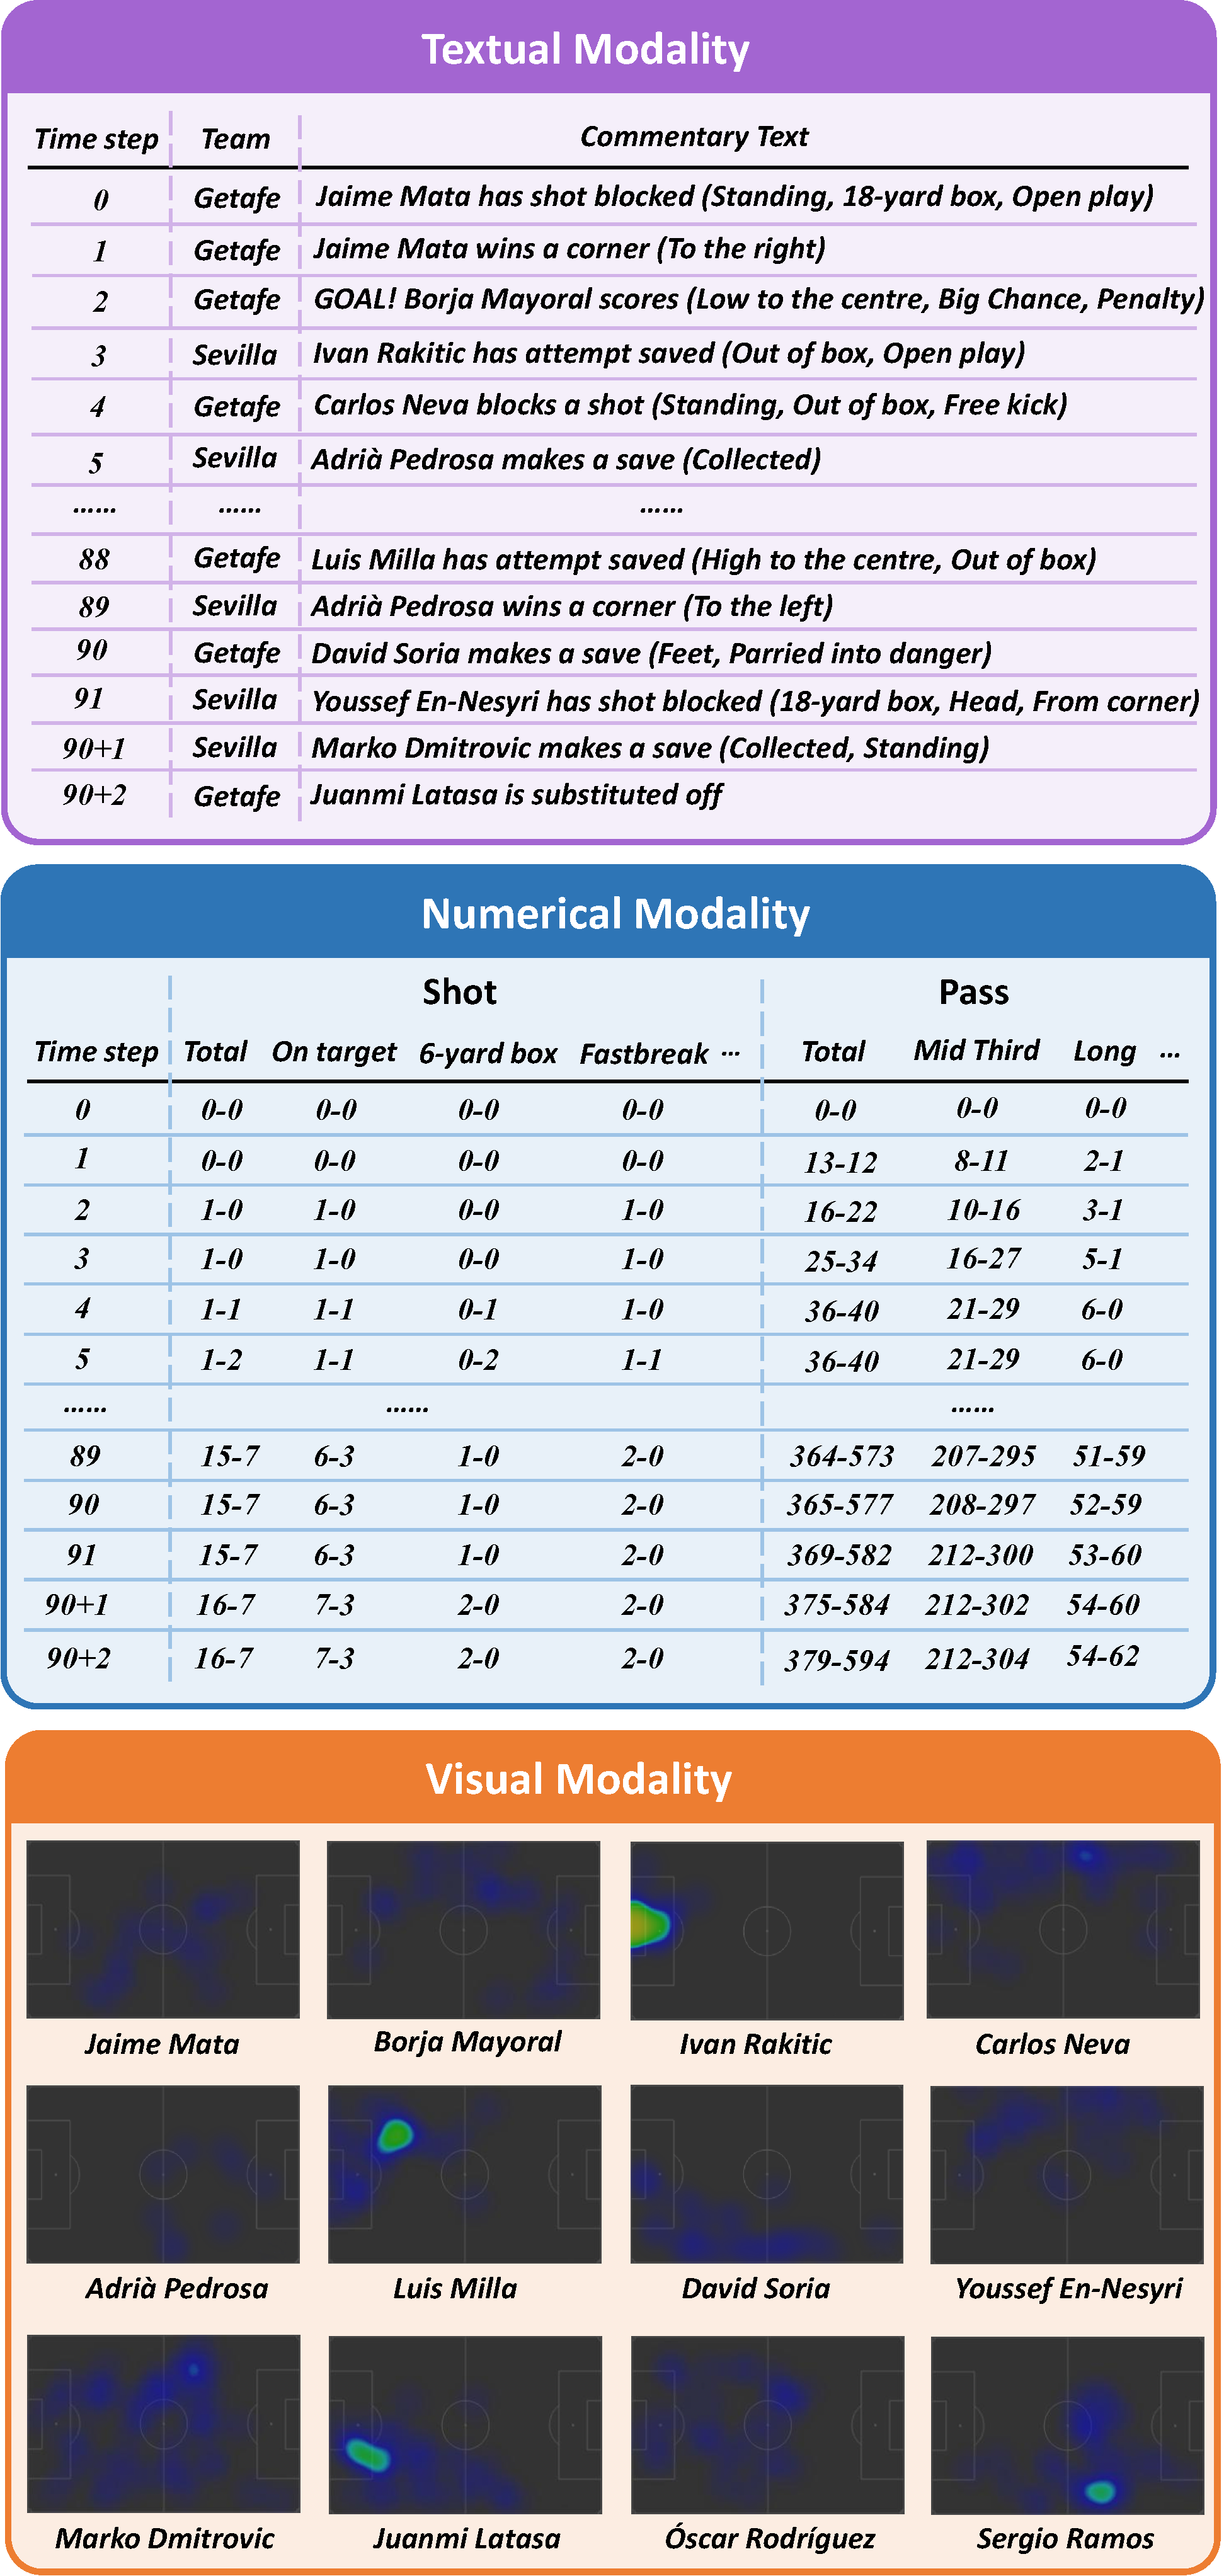
\includegraphics[width=\linewidth]{figure/ful2.pdf}
	\vspace{-5mm}
    \caption{Examples of three different modalities from a sample match.}
    \vspace{-4mm}
	\label{fig:data_introduction}
\end{figure}

WorldScope benchmark pairs low-level physical observations with high-level tactical style labels. All data are collected from the official website. \textbf{Textual modality:} We extract commentary texts from the \emph{Match Commentary} section of the \emph{Match Centre}. These texts provide descriptions of player actions (e.g., to the right, standing) and ball-related events (e.g., makes a save, wins a corner) at different time steps. \textbf{Numerical modality:} We extract fine-grained cumulative statistics at selected time steps from the \emph{Chalkboard} section of the \emph{Match Centre}. These metrics range from fundamental actions (e.g., passes and dribbles) to spatial and situational attributes (e.g., pitch zones and action direction). \textbf{Visual modality:} We collect positional heatmaps for all participating players from the \emph{Heatmaps} section of the \emph{Match Centre}, covering their spatial distribution over the full match. Figure~\ref{fig:data_introduction} illustrates an example from the three modalities.

These data are raw observations directly captured from the match and are therefore low-level in nature. Within each modality, individual data points are inherently fragmented: whether a single textual snippet, a discrete numerical update, or an isolated player heatmap, each observation remains only weakly interpretable in isolation. To overcome this, the model must integrate evidence across temporal and spatial dimensions within each modality to reconstruct the overall match narrative, rather than relying on simplistic single-feature shortcuts.

% A formal schema (field names, types, alignment with Match Centre exports, and normalization rules) will be inserted here when you finalize the release specification.

\subsection{The 12 Styles}
\label{app:twelve_styles}

The high-level outputs are directly extracted and unmodified from the \emph{Match Summary} section of the official \emph{Match Report}. Crucially, they are annotated by their domain experts, which eliminate any subjective bias or dataset tailoring. Through exhaustive data collection, we empirically verified that the platform's \textbf{domain experts annotate} matches using a closed set of exactly 12 discrete playing styles:

\textit{1). Played with width}

\textit{2). Favoured long shots}

\textit{3). Favoured short passing}

\textit{4). Attacked through the middle}

\textit{5). Favoured through balls}

\textit{6). Attacked down the left side}

\textit{7). Favoured crossing the ball}

\textit{8). Favoured long balls}

\textit{9). Had a high shot frequency when in possession}

\textit{10). Dominated possession}

\textit{11). Attacked down the right side}

\textit{12). Had a large quantity of possession in their opponent's half}

We explicitly define these 12 tactical styles as macroscopic targets because they represent latent strategic intentions rather than directly observable atomic events. None of these labels can be trivially extracted from a localized input occurrence or via superficial semantic shortcuts. Instead, correctly predicting any of these styles rigorously forces the model to execute the complete Understanding-Synthesizing-Reasoning (U/S/R) cognitive chain: First, in the Understanding (U) stage, the model must accurately ground isolated physical events, such as analyzing the efficiency of individual pass from numerical matrices or localized player densities from visual heatmaps. Next, in the Synthesizing (S) stage, it must integrate these fragmented, minute-by-minute atomic observations into a coherent, global spatial-temporal state—for instance, recognizing a persistent structural pattern where the ball is predominantly distributed along both flanks over the entire 90 minutes. Finally, in the Reasoning (R) stage, the model must transcend statistical counting to deduce the latent tactical philosophy, logically mapping this unified global dynamic to the specific strategic intentions.

% \textit{Played with width; Favoured long shots; Favoured short passing; Attacked through the middle; Favoured through balls; Attacked down the left side; Favoured crossing the ball; Favoured long balls; Had a high shot frequency when in possession; Dominated possession; Attacked down the right side; Had a large quantity of possession in their opponent's half}.

% Optional: per-label definitions, co-occurrence constraints, and annotation guidelines can be added in this subsection.

\begin{figure}[!t]
	\centering
	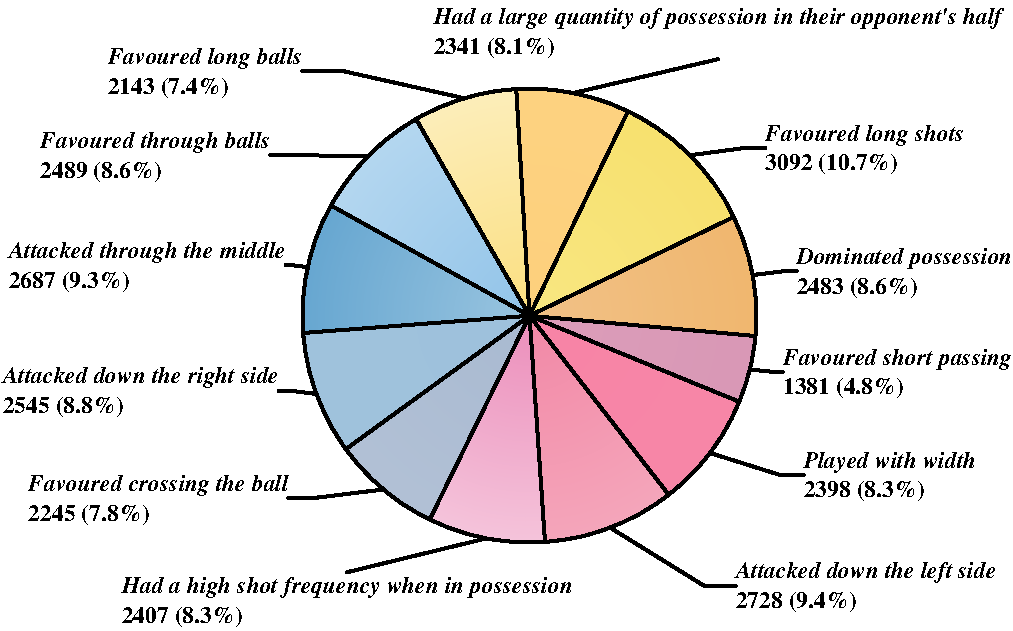
\includegraphics[width=\linewidth]{figure/new1.pdf}
	\vspace{-5mm}
    \caption{A pie chart showing the statistical data of playing styles in the dataset. It shows all the statements about playing styles, with their respective quantities and proportions.}
    \vspace{-4mm}
	\label{fig:evolution}
\end{figure}

\subsection{Data Statistics}
\label{app:data_stats}

Recordable matches from 2018 to 2023 were extracted via web crawling. During preprocessing, invalid records were identified and removed. For example, some matches contained incomplete commentary texts, missing statistical values, or lacked corresponding match reports. Importantly, this collection and filtering process is strictly architecture-agnostic. \textbf{We rely solely on automated web scraping and manual verification for data completeness, without any tailored feature engineering intended to favor models.} Furthermore, to ensure the semantic fidelity of the benchmark, we introduced a \textbf{rigorous human validation step}. Researchers familiar with football domain knowledge randomly sampled 20\% of the automatically filtered matches to manually verify the content quality—ensuring, for instance, that the scraped texts were genuine play-by-play commentaries rather than website artifacts, and that the multimodal observations logically corresponded to the annotated tactical styles. After this comprehensive cleaning and validation process, the final dataset contains complete records from 7 tournaments between 2018 and 2023. In total, 5,000 match records were retained and stored in JSON format. Unlike conventional multimodal datasets that often suffer from unbalanced modality distributions or missing paired data, WorldScope features strictly aligned cross-modal triplets. Specifically, each of the 5,000 match records is perfectly accompanied by all three heterogeneous inputs (textual commentary, numerical statistics, and visual heatmaps). This strict alignment results in 15,000 distinct input instances ($5,000 \times 3$ modalities) evaluated across the benchmark. Furthermore, these 5,000 holistic records are mapped onto the 12 expert-annotated tactical styles, offering a diverse and rich distribution of macroscopic targets for cognitive evaluation. This meticulously aligned scale and comprehensive label coverage provide a solid empirical basis for evaluating high-level cognition in models. We summarize the dataset scale in Table~\ref{fig:dataset_scale}.

% We summarize dataset scale and splits (e.g., train/test counts, per-modality coverage, label frequency, and sequence length statistics). \textbf{Placeholder:} insert tables or figures with your final numbers.

% \begin{table}[t]
%     \centering
%     \caption{Placeholder: MatchIntel2 statistics (splits, label distribution, sequence lengths, etc.).}
%     \label{tab:app_data_stats_placeholder}
%     \begin{tabular}{l c}
%         \toprule
%         \textbf{Statistic} & \textbf{Value (TBD)} \\
%         \midrule
%         Total examples & TBD \\
%         Train / Test split & 4{,}500 / 500 \\
%         Per-label frequency (12 styles) & TBD \\
%         Other (e.g., avg.\ timesteps per match) & TBD \\
%         \bottomrule
%     \end{tabular}
% \end{table}

% Table generated by Excel2LaTeX from sheet 'Sheet1'
\begin{table}[t]
  \centering
  \caption{Collection status of the dataset. The dataset covers 7 tournaments from 2018 to 2023.}
  \renewcommand\arraystretch{1.5} 
  \resizebox{\linewidth}{!}{
    \begin{tabular}{l|cccccc|c}
    \bottomrule
    \diagbox[width=15em,height=2.0em]{Tournaments}{Year} & 2018  & 2019  & 2020  & 2021  & 2022  & 2023  & Total \\
    \hline
    Premier League (England)     & 117 & 135 & 115 & 132 & 118 & 126 & 743 \\
    Serie A (Italy)              & 114 & 104 & 128 & 121 & 110 & 103 & 680 \\
    LaLiga (Spain)               & 141 & 116 & 118 & 120 & 108 & 117 & 720 \\
    Ligue 1 (France)             & 136 & 111 & 85  & 136 & 103 & 122 & 693 \\
    Bundesliga (Germany)         & 109 & 95  & 87  & 115 & 114 & 106 & 626 \\
    Brasileirão (Brazil)         & 146 & 141 & 103 & 187 & 137 & 147 & 861 \\
    Liga Profesional (Argentina) & 131 & 119 & 36  & 123 & 133 & 135 & 677 \\
    \hline
    Total                        & 894 & 821 & 672 & 934 & 823 & 856 & 5000 \\
    \toprule
    \end{tabular}%
    }
  \label{fig:dataset_scale}%
\end{table}%

\subsection{Construction Pipeline}
\label{app:construction_pipeline}

The construction of WorldScope follows a systematic data acquisition pipeline from the WhoScored platform. The strictly decoupled nature of the benchmark is inherent in the site's architecture, since the inputs and outputs are retrieved from independent functional modules:

\begin{itemize}[leftmargin=*]
    \item \textbf{Input Acquisition (Event-based):} The low-level multimodal data are crawled from the \textit{Match Centre} and \textit{Chalkboard} sections. These sections provide objective, real-time logs of the match (e.g., coordinate-based heatmaps, timestamped commentary, raw statistical counts, and player heatmaps). This information represents the raw physical process of the match.
    
    \item \textbf{Output Acquisition (Expert-based):} The high-level tactical labels are directly extracted from the \textit{Match Report} section. Unlike the raw objective logs, these reports provide macroscopic tactical evaluations generated post-match. Instead of parsing free-form summaries, we directly retrieve the explicitly identified ``Team Characteristics'', which are natively categorized by the platform into a finite set of 12 tactical playing styles.
\end{itemize}

To ensure rigorous evaluation, we maintain strict separation during crawling and pairing. The input features are restricted to \textit{what happened} (facts), while the output labels represent \textit{how it was played} (interpretations). By aligning these two independently crawled sources through Match IDs, we create a non-trivial gap between low-level observations and high-level conclusions, reducing the possibility of simple surface overlap.

% -----------------------------------------------------------------------------
% \clearpage
\section{Experiment Setup}
\label{app:experiment_setup}

\subsection{Models}
\label{app:models}
To comprehensively evaluate HWI-related capabilities and establish the empirical boundaries of both general intelligence and passive data fitting, we select a diverse and representative set of models. \textbf{Closed-Source State-of-the-Art Models:} To probe the current ceiling of commercial foundation models, we evaluate GPT-5.4 and Claude-4.6-opus. These models are accessed strictly via their official APIs and are tested across all three modalities. \textbf{Open-Weight LLMs:} For the textual and numerical modalities, we select prominent open-weight LLMs spanning various parameter scales to analyze potential scaling effects, including Llama-3.1 (70B), Mistral-Small-3 (24B), Qwen-2.5 (3B), and Vicuna-1.5 (7B). \textbf{Open-Weight VLMs:} To evaluate the visual modality, we utilize the corresponding multimodal variants of the aforementioned LLMs, namely Llama-3.2-Vision (90B), Mistral-Small-3.1 (24B), Qwen-2.5-VL (3B), and LLaVa-1.5 (7B). Crucially, the backbones of these VLMs are initialized from their corresponding text-only language models (e.g., Llama-3.2-Vision is built upon Llama-3.1, and Mistral-Small-3.1 is built upon Mistral-Small-3). This structural correspondence helps support a fairer cross-modal comparison when diagnosing the Modality Gap. Additionally, we fine-tune several representative LLMs on the training set, enabling a direct comparison against traditional architectures trained entirely from scratch. To ensure strict evaluation fairness across both training and inference stages, all models undergo rigorous \textbf{5-fold cross-validation} on the exact same data splits. This unified benchmarking guarantees that the observed performance gaps reflect genuine architectural capabilities rather than dataset bias. Full implementation and training details are provided below.

% This section consolidates model choices and training protocols referenced from Section~4. Hyperparameters are summarized in Appendix~\ref{app:parameters}.
\begin{figure*}[!t]
	\centering
	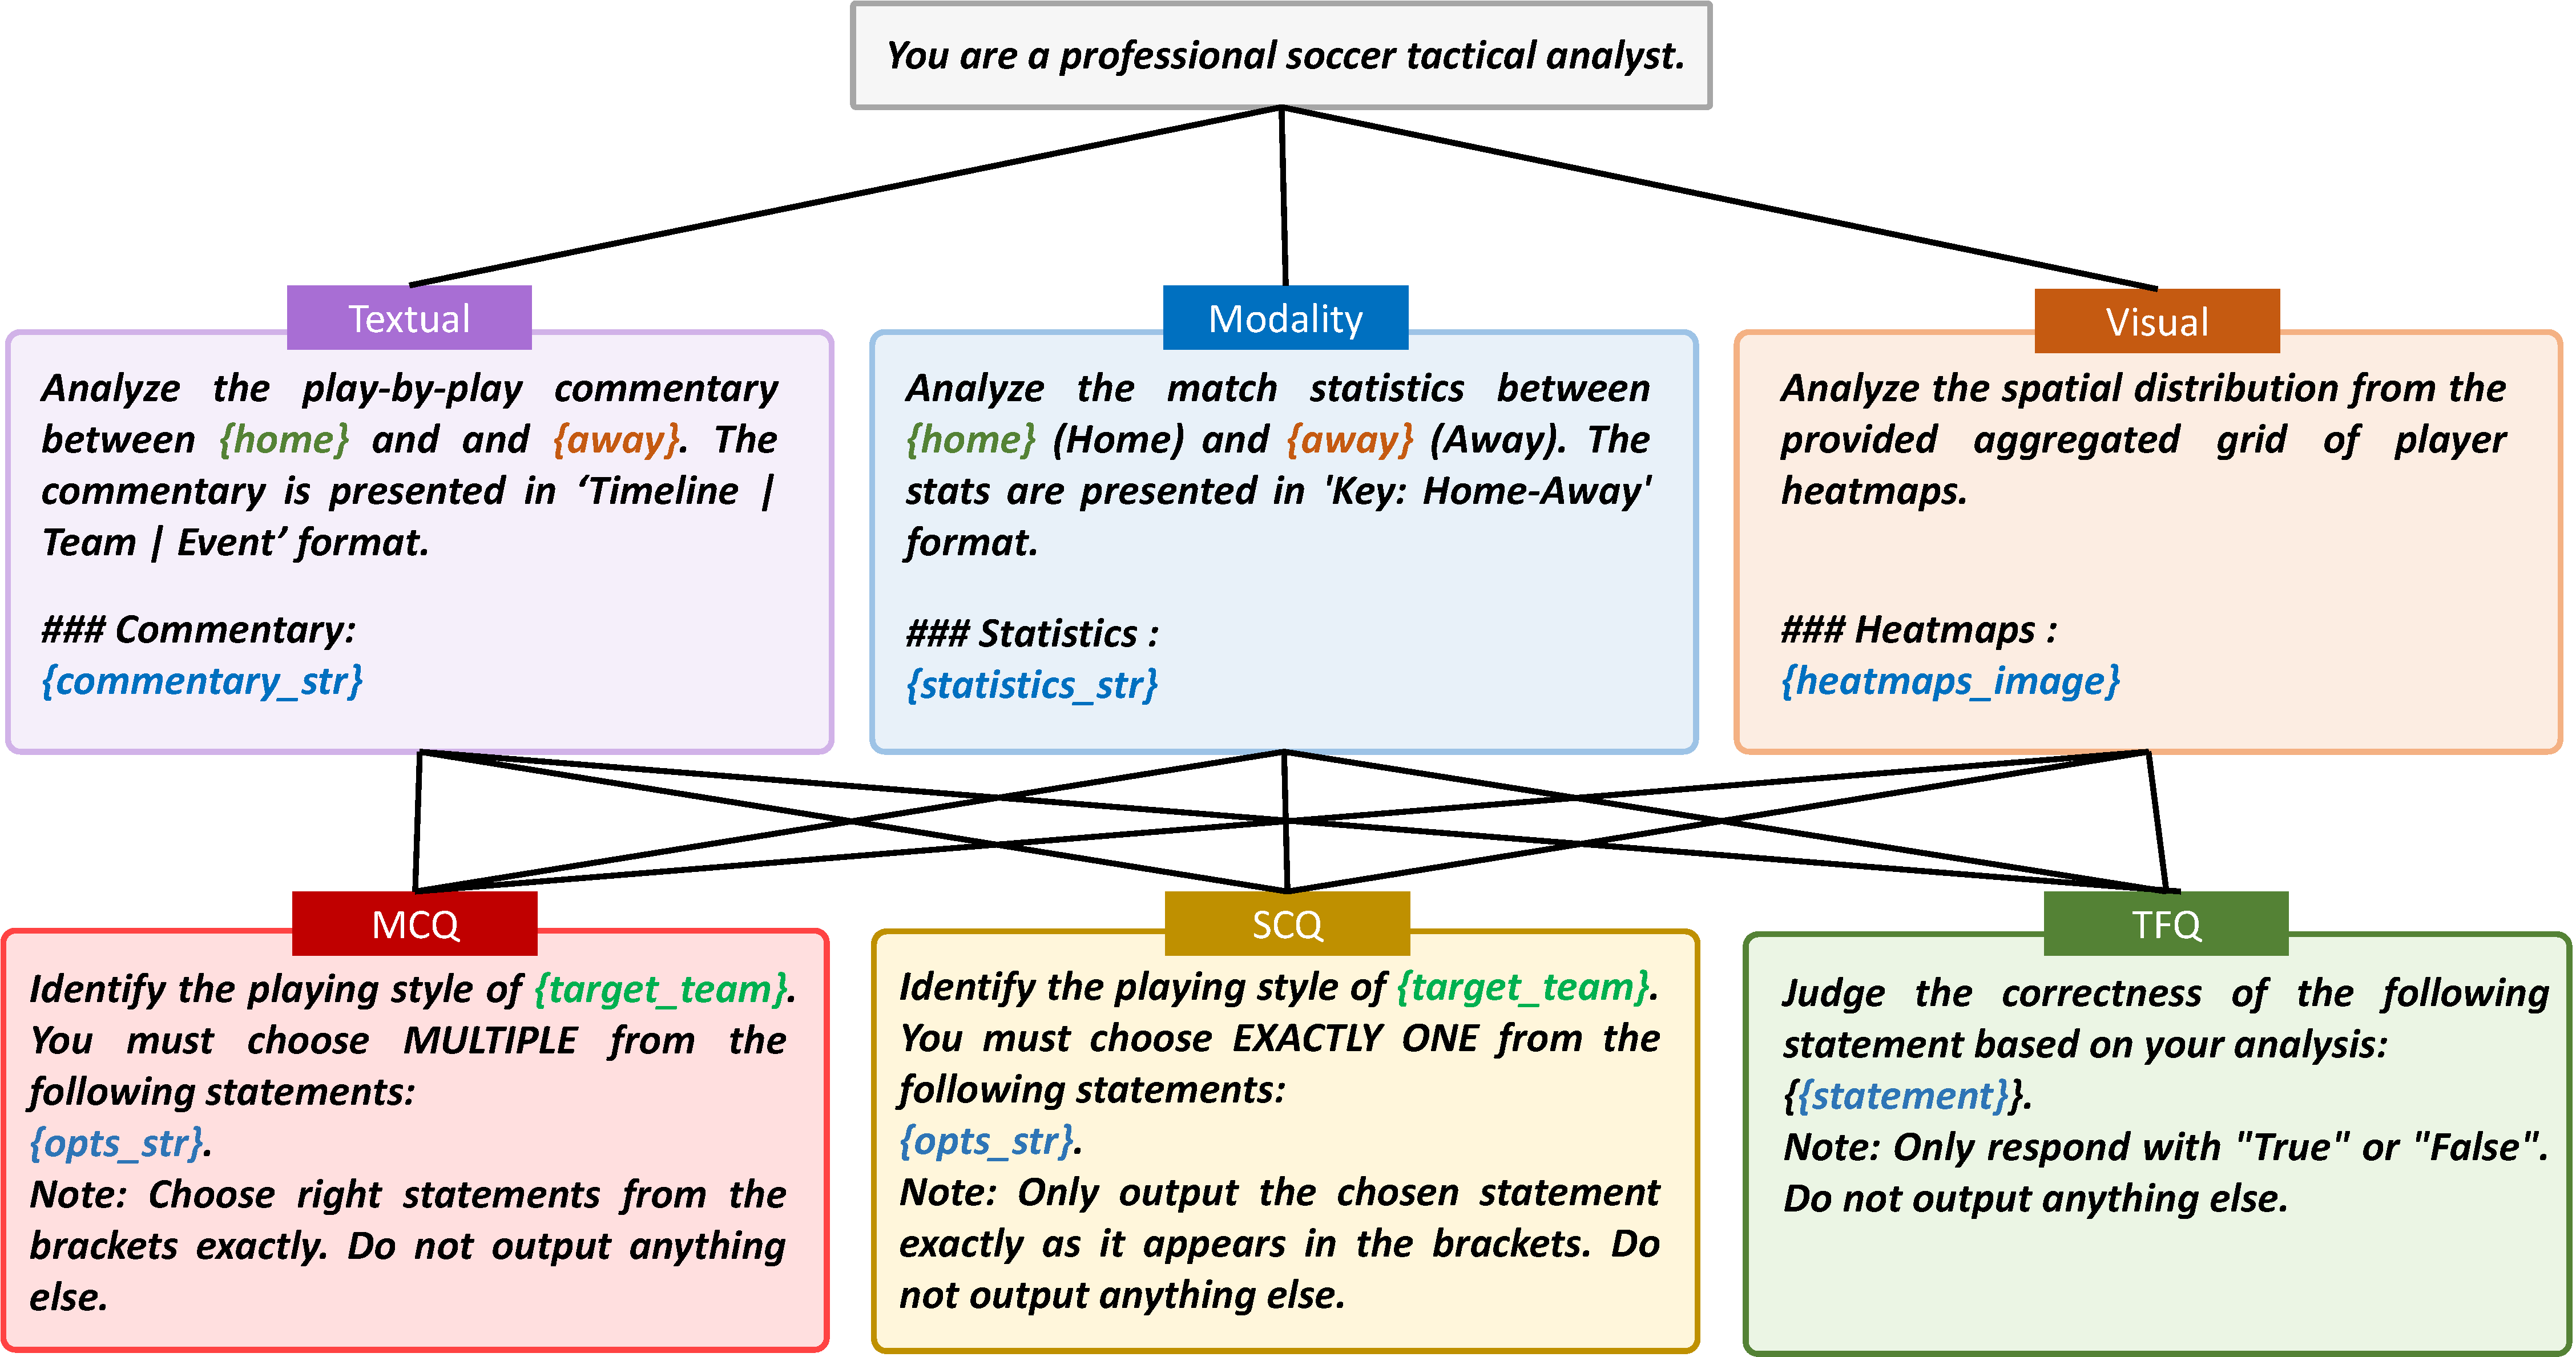
\includegraphics[width=\linewidth]{figure/figure23.pdf}
	\vspace{-5mm}
    \caption{Prompt design. First, the model is assigned the role of a soccer tactical analyst. Then, a task with a specified modality is provided, followed by a question in a specified format.}
    \vspace{-4mm}
	\label{fig:prompt}
\end{figure*}

\subsubsection{Fine-Tuning LLMs}
To adapt LLMs to the task, supervised fine-tuning (SFT) is performed on the collected dataset. Several models with strong instruction-following capabilities, specifically Qwen2-VL-2B, LLaVA-1.5-13B, Vicuna-13B-v1.5, and Qwen2.5-7B, serve as the foundation models across different modalities. To align with their input paradigms, the inputs are integrated into a unified conversational template. Specifically, for the visual modality, heatmaps are projected into the embedding space by vision encoders and aligned with fixed token placeholders, while fragmented numerical statistics are serialized into structured text for the textual and numerical modalities. This design allows LLMs to process the raw physical observations as conditional prefixes.

Additionally, to enable efficient fine-tuning, we adopt Quantized Low-Rank Adaptation (QLoRA). The foundation models are quantized to 4-bit precision using NormalFloat4 (NF4) with bfloat16 as the compute data type, and learnable Low-Rank Adapters (LoRA) are inserted into their linear projection layers, including both attention and MLP modules. During fine-tuning, the pre-trained weights remain frozen, and only the adapter parameters are updated through backpropagation. Training follows the standard causal language modeling paradigm, where models are trained to autoregressively generate high-level conclusions. The optimization minimizes the cross-entropy loss between the generated outputs and the ground-truth labels, strictly conditioned on the multimodal instruction context, with prompt tokens explicitly masked out from the loss.

\subsubsection{Training Traditional Architecture Models}
We train a suite of traditional architecture models to serve as rigorous baselines. These models bypass language-centric tokenization and process raw physical observations directly, aiming to predict the multi-label tactical styles of the target team.

For the textual modality, we introduce an event-driven framework to process the chronological play-by-play commentary. Each commentary event is tokenized and mapped to learned word embeddings. To handle varying sentence lengths, a masked average pooling mechanism is applied to extract a dense semantic representation for each text snippet. This textual feature is then concatenated with event-specific metadata, namely the normalized timestamp and binary team attribution, to construct a unified event vector that grounds the isolated text in the overall match context. To establish robust baselines, we independently train and evaluate three separate models on these sequences. The first, a pure Multi-Layer Perceptron (MLP), aggregates all events within a match via average pooling to form a global representation. In parallel, two bidirectional sequence models, GRU and LSTM, are trained individually to trace the chronological progression and contextual evolution of the match. These temporal models apply max pooling across the sequence dimension to extract the most decisive textual highlight signals associated with high-level tactical intents.

For the numerical modality, we design three distinct architectures to process the statistical data. The first is a hierarchical 1D Convolutional Neural Network (1D CNN) consisting of three consecutive convolutional blocks with batch normalization and ReLU activation, progressively expanding channel dimensions to extract local short-term dependencies from the sequential statistics. The second is a Delta-GRU model, which computes discrete differences across sequential milestones to capture the temporal evolution of match statistics. These dynamic variations are processed through a bidirectional Gated Recurrent Unit (GRU) and aggregated via a dual-pooling mechanism that concatenates adaptive average pooling and max pooling. The third is a pure Multi-Layer Perceptron (MLP) baseline that directly flattens the multi-step feature sequences into a unified vector. For all three architectures, the final aggregated representations are fed into a fully connected classifier to map the extracted patterns to multi-label predictions.

For the visual modality, we formulate the task as a Multiple Instance Learning (MIL) problem, where a complete match is treated as a bag of sequential heatmaps representing spatial activity zones over time. To comprehensively evaluate visual feature extraction, we employ three distinct shared instance-level encoders: ResNet-18, DenseNet-121, and EfficientNet-B0. Each backbone projects individual heatmap instances into high-dimensional feature vectors. Subsequently, a permutation-invariant max-pooling operation is applied across the instance dimension to aggregate these features into a unified representation. This design ensures that the most decisive signals for high-level outcomes can be retained without dilution, regardless of the specific time step at which they occur. The aggregated representation is then passed through an MLP classification head.

Finally, all traditional architecture models across the three modalities are optimized using binary cross-entropy loss.


\subsection{Parameters}
\label{app:parameters}

\subsubsection{Fine-Tuning Details and Hyperparameters}
LLMs are fine-tuned using 4-bit QLoRA ($r=64$, $\alpha=16$) for 5 epochs with the 32-bit Paged-AdamW optimizer. To accommodate the distinct characteristics of different modalities, hyperparameters are tailored accordingly: for visual tasks, the learning rate is set to $1\times10^{-4}$ with a dropout rate of 0.05 and a weight decay of 0.01; for numerical and textual tasks, the learning rate is $2\times10^{-4}$ with a dropout rate of 0.1 and a weight decay of 0.001. All models are trained with a warmup ratio of 0.03, a per-device batch size of 1, 8 gradient accumulation steps, and bfloat16 (BF16) precision.

% \subsubsection{Trained-from-Scratch Parameters}

\subsubsection{Implementation Details and Hyperparameters}
The traditional architecture models are optimized using the Adam optimizer and Binary Cross-Entropy (BCE) loss across all modalities. \textbf{Textual Modality:} The \texttt{bert-base-uncased} tokenizer is employed to process the commentary texts. To standardize the inputs, the sequences are capped at a maximum of 150 events per match and 32 words per event, with an embedding dimension of 128. These textual models are trained with a batch size of 16 and a learning rate of $10^{-3}$. \textbf{Numerical Modality:} Statistical sequences are constructed using 15-minute milestone intervals. All numerical architectures are trained with a batch size of 32 and an initial learning rate of $10^{-3}$, modulated by a cosine annealing learning-rate scheduler to ensure stable convergence. \textbf{Visual Modality:} Input heatmaps are resized to $215 \times 329$, with each MIL bag containing up to 18 instances representing the match evolution. To accelerate training while maintaining numerical stability, Automatic Mixed Precision (AMP) is employed. All visual models are optimized with a learning rate of $10^{-4}$.

\subsubsection{Inference Hyperparameters of LLMs}
To ensure stable generation of valid answers, we adopt nearly deterministic decoding settings. Specifically, the temperature is set to $10^{-4}$ and top-$p$ is set to 1.0.



\subsection{Prompt Design}
\label{app:prompts_zeroshot_fewshot}

For zero-shot evaluation, we design fixed instruction templates for each modality to help the language models interpret the distinct data formats and evaluate the task without cross-modal interference. Crucially, to verify model interface compatibility, we conducted a pre-task comprehension sanity check before the formal evaluation. When fed raw isolated inputs without downstream QA tasks and prompted to simply describe them, the evaluated LLMs and VLMs successfully identified the data structures (e.g., explicitly describing a visual input as a football player's positional heatmap or a text sequence as match commentary). This confirms that the models possess the fundamental capability to parse these low-level physical representations, thereby guaranteeing that our benchmark genuinely evaluates their endogenous cognitive abilities rather than mere interface incompatibility. \textbf{Textual Modality:} The context provides play-by-play commentary structured in a strictly chronological \texttt{Timeline | Team | Event} format. This sequential structure preserves the temporal dynamics of the match, enabling the model to trace tactical shifts and game momentum over time. \textbf{Numerical Modality:} The context presents time-series match statistics aggregated at specific milestones. The data are serialized into a structured \texttt{Key: Home-Away} format, allowing the model to directly quantify comparative team performance and event frequencies from discrete numerical indicators. \textbf{Visual Modality:} The model is instructed to evaluate spatial distributions derived from an aggregated grid of individual player heatmaps. This visual prompt encapsulates complex player activities into a single image, guiding the vision encoder to focus on spatial relationships and zonal dominance.

\textbf{Robustness via Diverse Task Formulations:} Following the modality-specific context, a standardized task query is appended. To rigorously evaluate the robustness of the models' cognitive capabilities and ensure that their performance is not an artifact of prompt engineering, we dynamically construct three distinct evaluation formats for \textit{each} test sample: 

\begin{itemize}
    \item \textbf{MCQ (Multiple-Choice Question):} Extract two to four appropriate playing styles from four candidates.
    \item \textbf{SCQ (Single-Choice Question):} Select one correct playing style from four candidates.
    \item \textbf{TFQ (True/False Question):} Judge whether a presented style set is absolutely correct.
\end{itemize}

By exposing the exact same physical sample to multiple heterogeneous question formats, we strictly test the models' robustness. A model possessing genuine high-level cognition must demonstrate consistent tactical deduction regardless of how the inquiry is formulated. To facilitate automated evaluation, these task queries require the model to output only deterministic answers (e.g., the exact option string or a boolean value). The prompts are shown in Figure~\ref{fig:prompt}. For few-shot learning, 1 to 2 high-quality demonstration examples are appended before the final query. Each demonstration pairs the corresponding intra-modality context with its reasoning process and final answer, thereby guiding the model's output distribution toward the expected response format through in-context learning.


% \subsection{Zero-Shot and Few-Shot Prompt}
% \label{app:prompts_zeroshot_fewshot}

% Zero-shot evaluation uses fixed instruction templates aligned with prior textual HLC work, with commentary replaced by numerical or visual inputs. Few-shot variants append 1--2 demonstration examples before the query. \textbf{Placeholder:} paste full prompt templates (per modality and per assessment format) here for reproducibility.


% Lightweight models are trained from scratch. The 1D CNN employs the Adam optimizer (lr=$10^{-3}$, kernel sizes $\{3, 5, 7\}$), and MIL-ResNet-18 processes the heatmaps (up to 18 images) using an ImageNet-pretrained backbone.

% -----------------------------------------------------------------------------
% \clearpage
\section{Case Studies}
\label{app:Case Studies}
This section presents several typical case studies to provide an deep analysis of the limitations of  LLMs in handling high-level cognition tasks. These cases cover errors in three representative reasoning tasks (MCQ, SCQ, TFQ), as well as severe failure scenarios such as generating completely irrelevant text. Figure \ref{fig:failure1}\textasciitilde \ref{fig:failure4} illustrate these failure patterns.
% \subsection{Models}
% \label{app:models}



% \subsection{Per-Class Accuracy}
% \label{app:per_class_accuracy}

% \textbf{Placeholder:} report per-style precision/recall or accuracy breakdown (e.g., macro-F1 per label) for each model family and modality.

% \begin{table}[t]
%     \centering
%     \caption{Placeholder: per-class metrics (12 styles $\times$ models).}
%     \label{tab:app_per_class_placeholder}
%     \begin{tabular}{l c c c}
%         \toprule
%         \textbf{Style / Model} & \textbf{Num.} & \textbf{Vis.} & \textbf{Notes} \\
%         \midrule
%         \multicolumn{4}{c}{\textit{TBD}} \\
%         \bottomrule
%     \end{tabular}
% \end{table}

% \subsection{Qualitative Case Study}
% \label{app:case_study}



% -----------------------------------------------------------------------------
% \clearpage
\section{Limitations \& Future Work}
\label{app:limitations_future}
\label{sec:limitations}

\subsection{Limitations}
\label{app:limitations}

Although this work provides critical insights into the capability boundaries of current large models, it is still subject to several limitations. First, while our zero-shot evaluations benchmark models with sizes up to 90B parameters, our fine-tuning experiments are constrained by computational resources and therefore focus on open-weight models up to 13B parameters. Although this scale is already sufficient to reveal the lack of endogenous structural growth in current LLMs under our setting, extending dynamic training to hundred-billion-parameter scales could further clarify the extreme boundaries of the observed Modality Gap. 

Second, to operationalize the HWI framework, the current WorldScope benchmark instantiates physical-world observations through three discrete channels: textual, numerical, and visual. However, the physical world inherently contains richer and more continuous signals, such as audio and temporal sensorimotor streams, which remain outside the scope of the present study. 

Third, to rigorously isolate and diagnose Modality-Agnostic properties, our current protocol evaluates the U/S/R cognitive chain by integrating fragmented data strictly within a single modality at a time. As a result, the more challenging setting of simultaneous cross-modality integration is not addressed in the current version of the benchmark.

\subsection{Future Work}
\label{app:future_work}

Addressing these limitations forms the trajectory of our future research. First, we plan to expand WorldScope into a more comprehensive benchmark that covers a broader spectrum of non-semantic and continuous physical modalities. Second, we will extend the current cognitive evaluation pipeline from single-modality reasoning to more complex cross-modality fusion, testing whether models can synthesize disjoint local states from heterogeneous channels into a unified global representation. 

Finally, to move beyond the capability collapse associated with passive data-fitting paradigms, we will explore the integration of specialized inductive biases and neuroplasticity-inspired architectures into LLMs. Ultimately, our goal is to equip foundation models with the capacity for authentic U$\rightarrow$S$\rightarrow$R cognition and sustained Open-ended Evolution, reducing their reliance on textual semantic shortcuts and bringing them closer to genuine world-grounded intelligence.

% \subsection{Limitations}
% \label{app:limitations}

% Constrained by available computational resources, fine-tuning focuses on open-weight models with parameter sizes up to 13B. These results support the absence of reliable MHLC in general LMs under our protocol, but larger scales could further validate the modality gap. The evaluation is conducted in numerical and visual modalities as representatives of non-semantic features; many physical-world signals (e.g., audio, sensorimotor streams) remain outside this study.

% \subsection{Future Work}
% \label{app:future_work}

% We plan to expand the evaluation framework into a broader non-semantic benchmark and to explore integrating specialized inductive biases into large-scale models so that U$\rightarrow$S$\rightarrow$R cognition can be realized without relying on textual semantic shortcuts.

% -----------------------------------------------------------------------------
% \clearpage
\section{U/S/R Error Attribution Rules}
\label{sec:usrules}

To move beyond the limitations of holistic performance metrics and provide a more granular diagnosis of model capabilities, we propose a systematic error-attribution protocol. Inspired by recent diagnostic methodologies that use rule-based verification frameworks to trace logical bottlenecks in language models \cite{mukherjee2026red,rafailov2023direct,zhiren2026learning}, we formalize the evaluation of the Understanding--Synthesizing--Reasoning (U/S/R) chain. Rather than relying on opaque heuristics, our protocol maps incorrect predictions to specific cognitive fractures using deterministic, bottom-up criteria derived from the model's raw output behavior:

\textbf{Understanding (U) Failure: Instruction Adherence and Grounding Collapse.} This foundational error is triggered when the model fails to extract the basic task semantics or to adhere to the explicitly specified output constraints. In our framework, the prompt strictly restricts the output to a predefined space of 12 tactical styles. A \textbf{U-fail} is recorded if the model generates unparseable text, conversational filler that violates the required format, or labels outside the candidate set. Such behavior indicates a fundamental collapse at the perception and grounding stage: the model is overwhelmed by the fragmented inputs and fails to recognize even the basic boundaries of the task.

\textbf{Synthesising (S) Failure: Internal Logical Dissonance via Mutual Exclusivity.} If the model successfully adheres to the output format and selects labels from the valid candidate set (thus passing the U stage), we then evaluate its internal consistency. Among the 12 tactical styles, certain subsets correspond to fundamentally contradictory physical states in football dynamics. For instance, a model that predicts both \textit{Favoured short passing} and \textit{Favoured long balls}, or simultaneously outputs \textit{Attacked through the middle} and \textit{Played with width}, exhibits a clear logical conflict. An \textbf{S-fail} is therefore assigned when the generated output contains such mutually exclusive label pairs. This indicates that, although the model can parse local events, it fails to synthesize them into a coherent and non-contradictory global interpretation.

\textbf{Reasoning (R) Failure: High-Level Semantic Misalignment.} The final stage of attribution occurs when the model produces an internally consistent and properly formatted output (passing both the U and S stages), yet the predicted tactical styles do not match the expert-annotated ground truth. An \textbf{R-fail} therefore isolates the error to the highest cognitive level. It indicates that the model is capable of perceiving the raw data and constructing a logically coherent scenario, but lacks the domain-specific reasoning ability required to map this synthesized world state to the correct macroscopic tactical conclusion.

\textbf{Implementation Details.} During evaluation, the model's raw output string is first parsed using regular expressions to match the 12 predefined style strings. The resulting predictions are then passed through an automated diagnostic pipeline: checking format adherence at the U stage, validating against a predefined matrix of mutually exclusive style pairs at the S stage, and finally comparing against the ground-truth labels via Exact Match at the R stage. This strict cascade ensures that the error attribution is mutually exclusive and collectively exhaustive.



\begin{figure*}[!t]
	\centering
	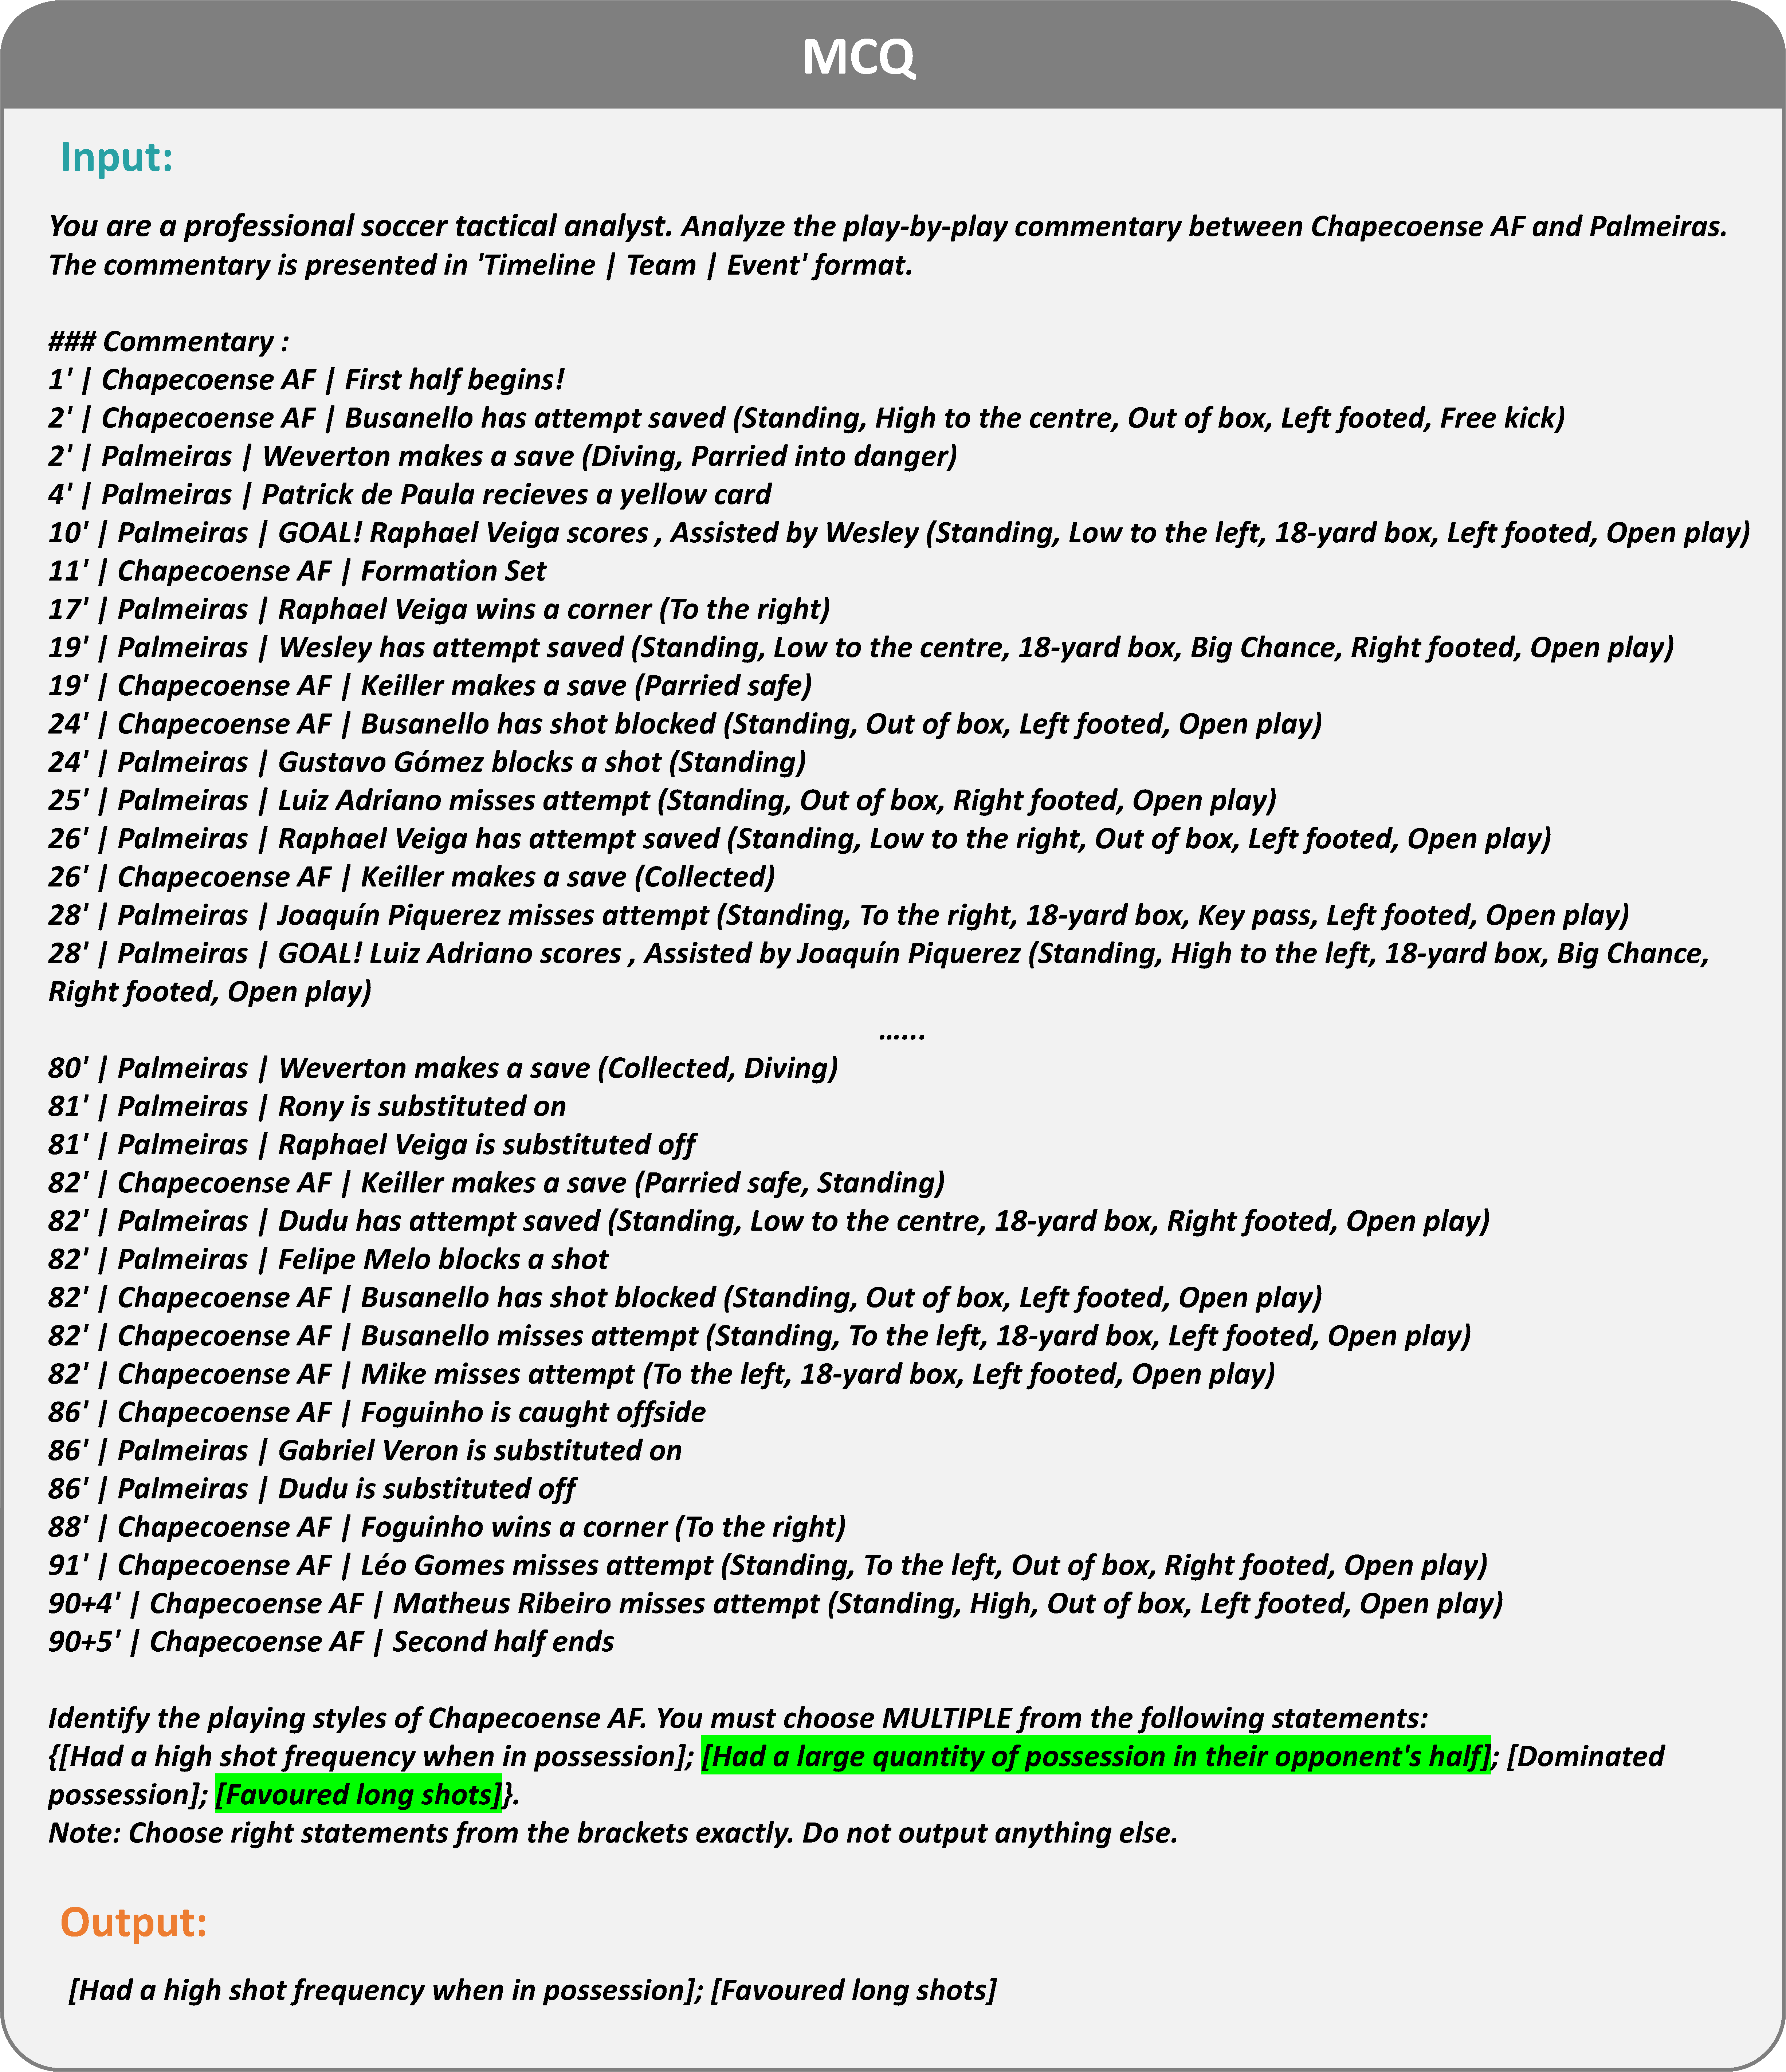
\includegraphics[width=\linewidth]{figure/figure31.pdf}
	\vspace{-5mm}
    \caption{This is a failure example of MCQ. The green sentences represent the ground truth, and the model's output does not perfectly match the ground truth. Note: Due to the length of the commentary, this example only shows a portion.}
    \vspace{-4mm}
	\label{fig:failure1}
\end{figure*}



\begin{figure*}[!t]
	\centering
	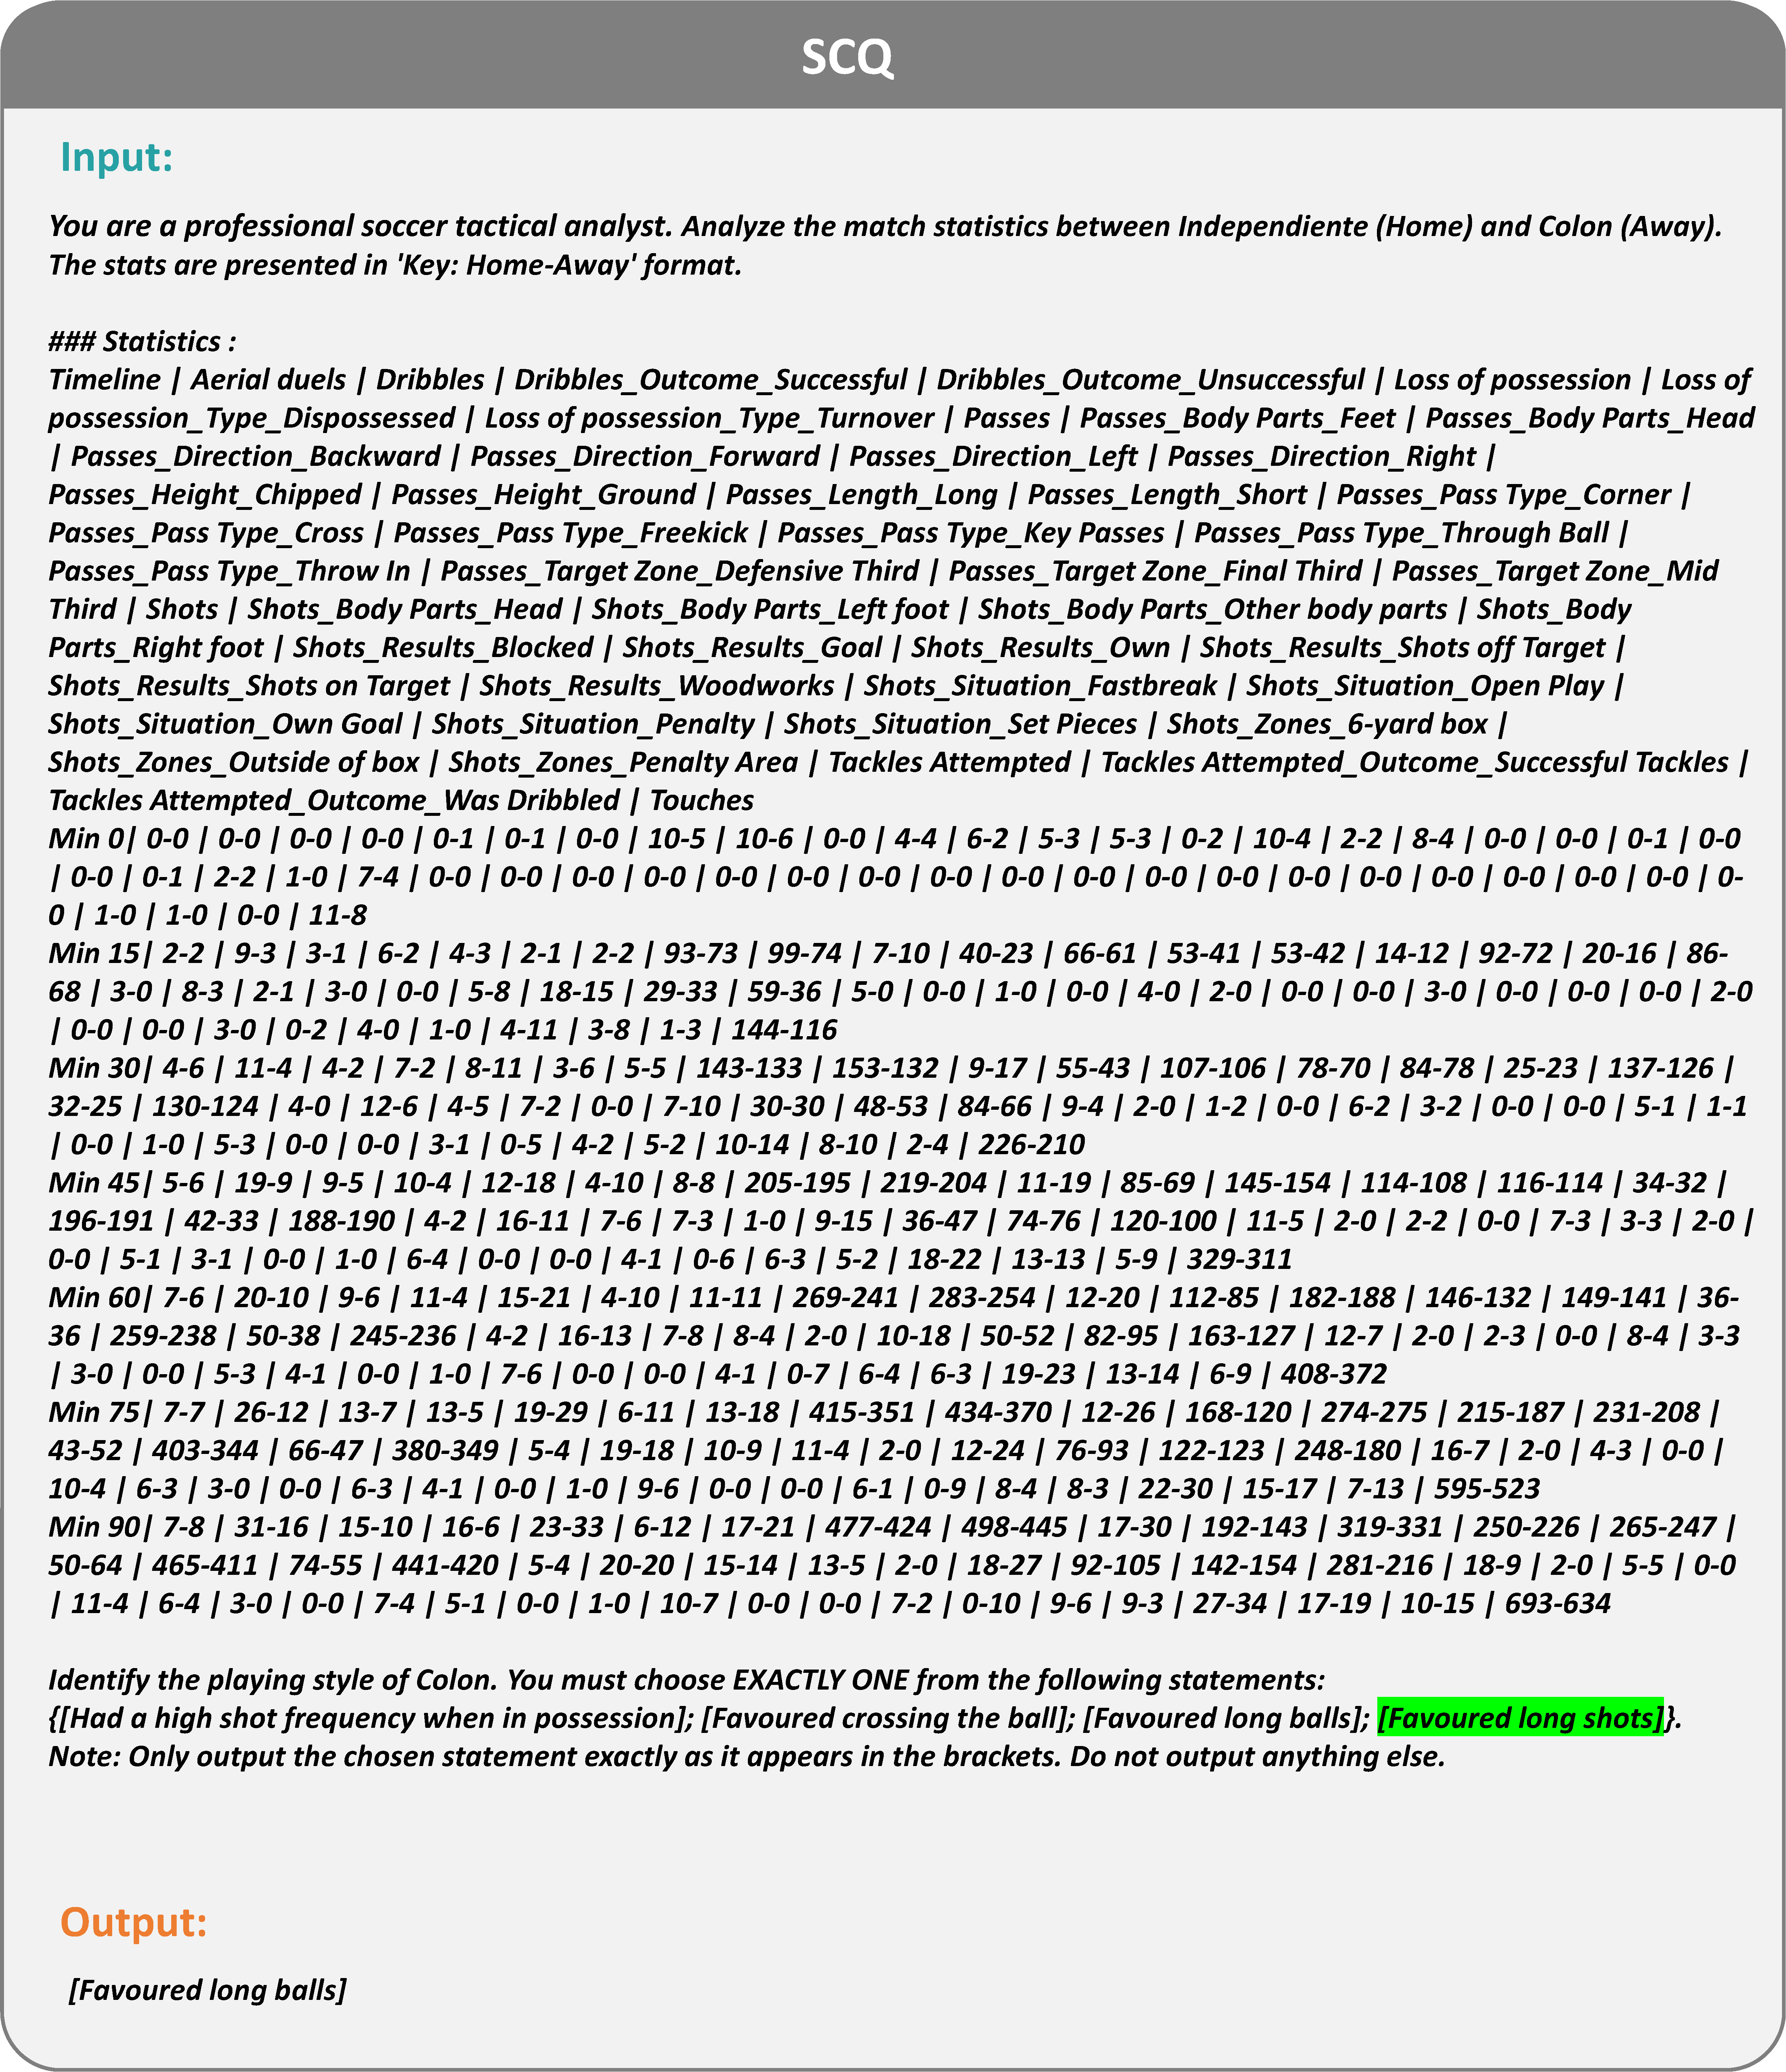
\includegraphics[width=\linewidth]{figure/figure32.pdf}
	\vspace{-5mm}
    \caption{This is a failure example of SCQ. The green sentences represent the ground truth, and the model's output does not match the ground truth.}
    \vspace{-4mm}
	\label{fig:failure2}
\end{figure*}

\begin{figure*}[!t]
	\centering
	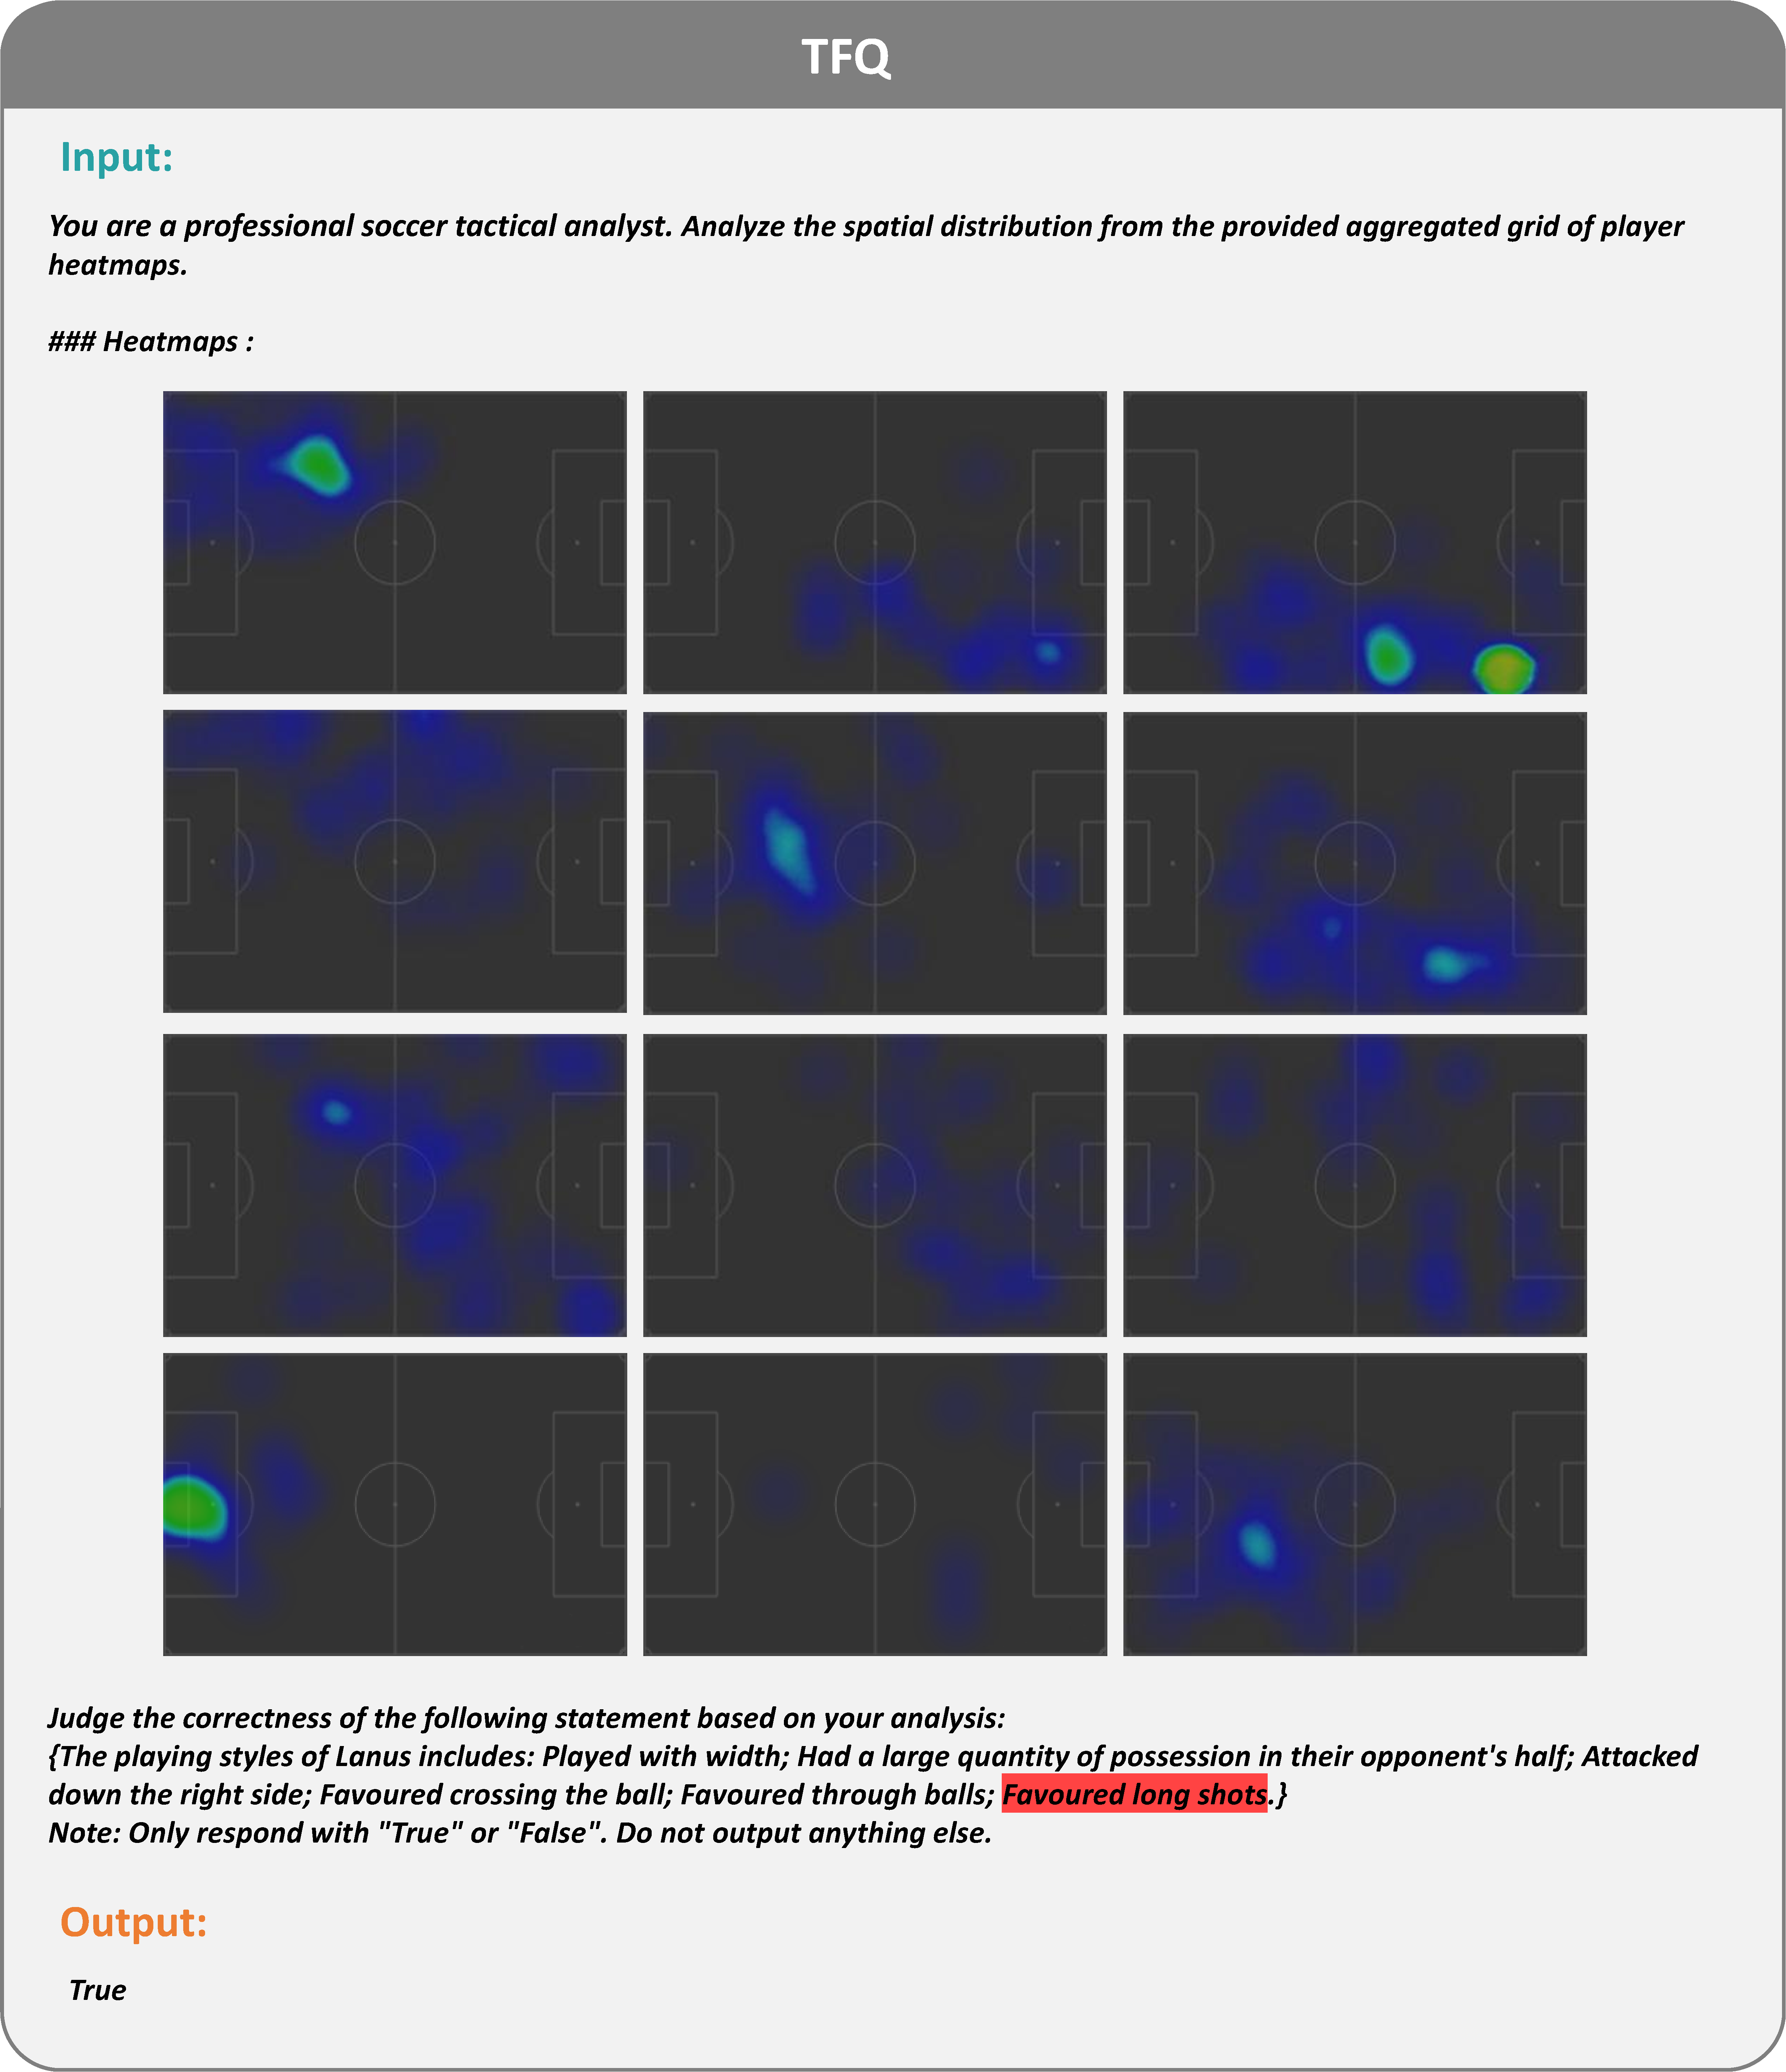
\includegraphics[width=\linewidth]{figure/figure34.pdf}
	\vspace{-5mm}
    \caption{This is a failure example of TFQ. The red sentences represent an incorrect style, but the model does not correctly identify it and considers the statement to be correct.}
    \vspace{-4mm}
	\label{fig:failure3}
\end{figure*}

\begin{figure*}[!t]
	\centering
	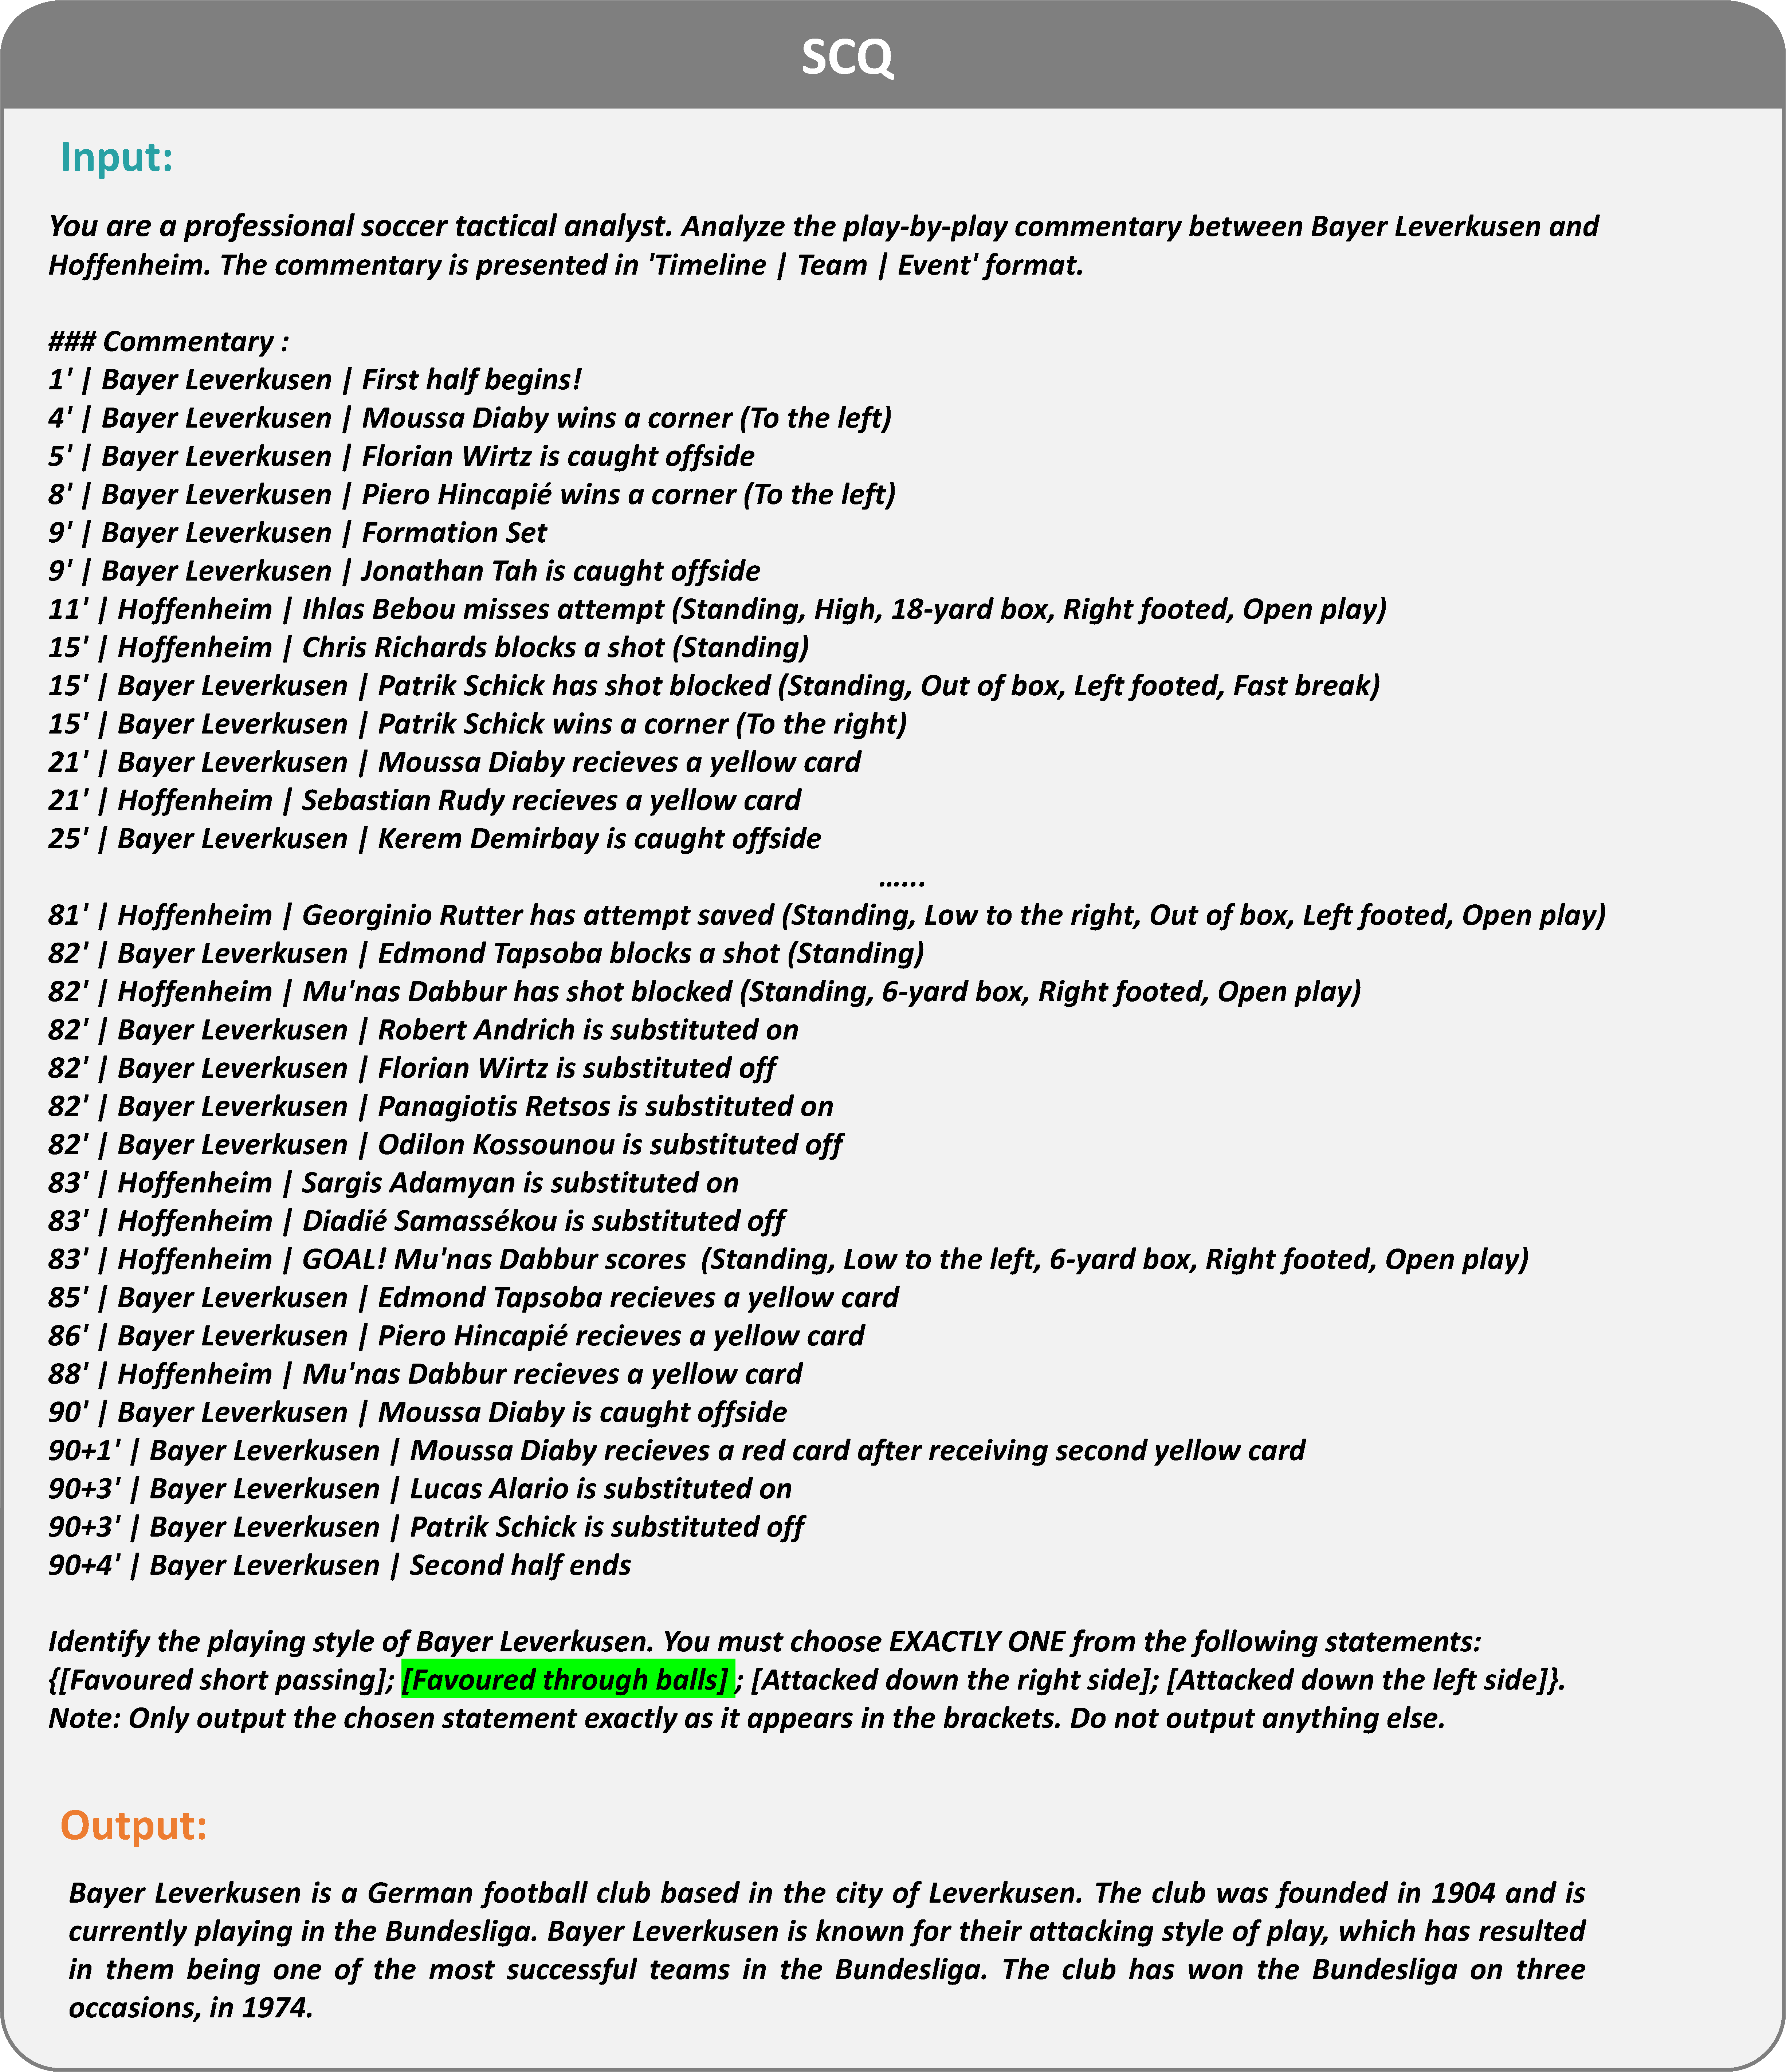
\includegraphics[width=\linewidth]{figure/figure35.pdf}
	\vspace{-5mm}
    \caption{This is a failed example with invalid output. The model is asked to perform SCQ, but its output is irrelevant text.}
    \vspace{-4mm}
	\label{fig:failure4}
\end{figure*}
